\documentclass{article}

\usepackage{fullpage,amsmath,amsthm,graphicx,enumitem}
\usepackage{hyperref}
\usepackage{amssymb}
\usepackage{wasysym}
\usepackage{empheq}
\usepackage{booktabs}

%For Grid, thanks internet: https://tex.stackexchange.com/questions/247541/help-with-grid-lines-in-a-pgfplot
\usepackage{tikz}
\usepackage{pgfplots}
\usetikzlibrary{calc}

\theoremstyle{definition}
\newtheorem{question}{Question}

\title{ASEN 3728 Aircraft Dynamics\\Written Homework 7}

\date{Due date listed on Gradescope.}

\begin{document}

\maketitle

\begin{question}
    Suppose that you are on the design team for what will become the Convair 880. The aircraft parameters are shown below:
\begin{figure}[htbp]
    \centering
    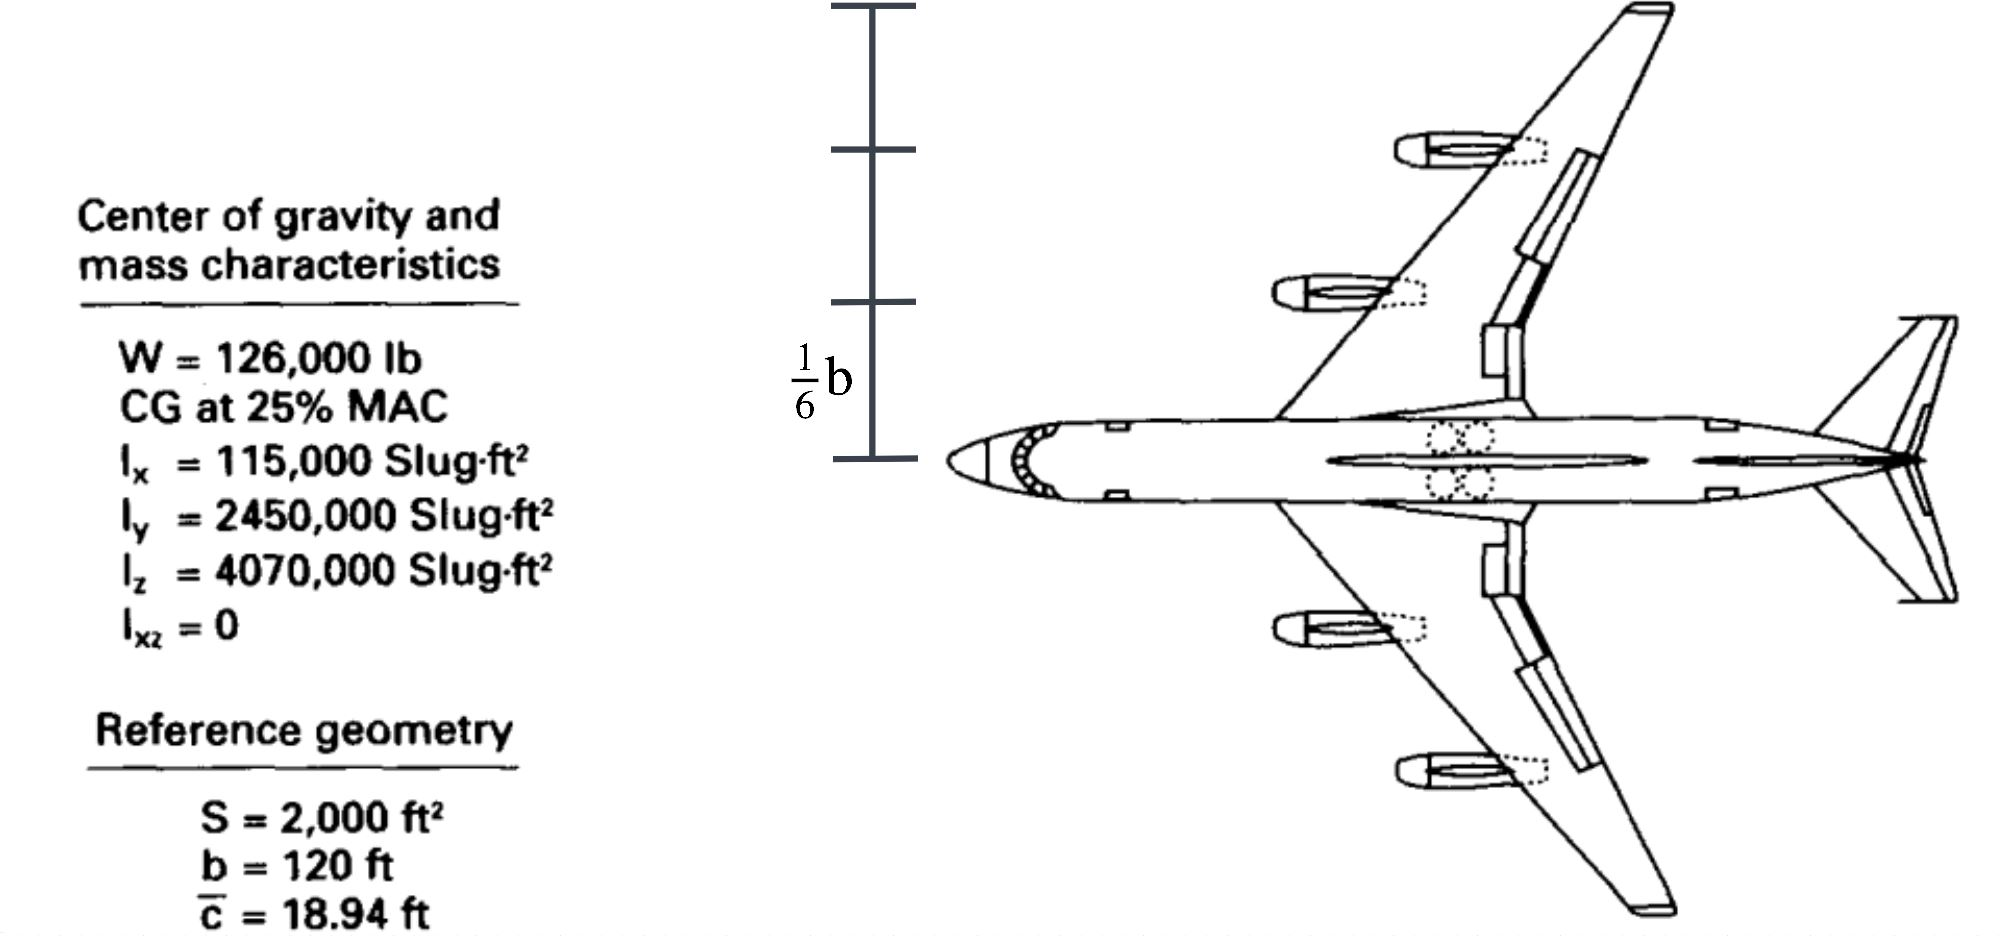
\includegraphics[width=0.85\textwidth]{convair880.jpg}
\end{figure}
\begin{table}[htbp]
    \centering
    \caption{Lateral stability derivatives for the Convair 880 at sea level.}
    \begin{tabular}{cccccccccccc} % Adjust column alignment as needed
        \toprule
$C_{y_\beta}$ & $C_{l_\beta}$ & $C_{n_\beta}$ & $C_{l_p}$ & $C_{n_p}$ & $C_{l_r}$ & $C_{n_r}$ & $C_{l_{\delta_a}}$ & $C_{n_{\delta_a}}$ & $C_{y_{\delta_r}}$ & $C_{l_{\delta_r}}$ \\ % $C_{n_{\delta_r}}$ \\
-0.877 & -0.196 & 0.139 & -0.381 & -0.049 & 0.198 & -0.185 & -0.038 & 0.017 & 0.216 & 0.0226 \\ % & -0.096 \\ 
    \bottomrule
    \end{tabular}
\end{table}

\begin{enumerate}[label=\alph*)]
    \item If the aircraft operates with $C_L = 0.68$ and $C_D = 0.08$ what is minimum thrust that this aircraft must apply to remain in trim assuming that thrust is directly opposed to drag.
    
    \item Consider the case where the leftmost engine suddenly loses power. The pilot wants to reduce the moment induced by the resulting asymmetry; however, the maximum thrust a single engine can contribute is $6000 \text{lb}_f$. What is the minimum yawing moment, $\Delta N_\text{thrust}$, that can be achieved by adjusting the individual throttles while maintaining the same total thrust? 

    \item Use a linear approximation to estimate the rudder power ($C_{n_{\delta_r}}$) needed so that flight with no sideslip can be maintained with an absolute rudder deflection of $3^\circ$ in this one-engine-out case.

    \item Use a linear approximation to estimate the aileron deflection and sideslip angle \textbf{in degrees} that would be needed to attain a steady flight condition in this one-engine-out case without any rudder deflection.

    
\end{enumerate}
\end{question}

\vspace{0.1cm}
\clearpage

\begin{question}
    While flying near sea-level at $u_0 = 10$ m/s with $\theta_0 = 0$, the TTwistor aircraft from homework P3 has the lateral dynamics matrix shown below. For all parts, show work and/or describe any code used.
    \begin{align*}
        \mathbf{A}_{lat} = 
        \begin{bmatrix}
         -0.2472 & -0.0671 & -9.7797 & 9.8100 \\
         -0.7966 & -16.5375 & 1.8114 & 0 \\
         0.4607 & -0.3451 & -0.4586 &  0 \\
         0 & 1.0000 & 0 & 0
        \end{bmatrix}
    \end{align*}
    \begin{enumerate}[label=\alph*)]
        \item Find the time constant of the roll mode, time constant of the spiral mode, and natural frequency and damping ratio of the Dutch roll mode of the TTwistor using the full lateral matrix. \label{part:4by}
        \item Calculate the time constant of the roll mode using the roll mode approximation. Compare this to the time constant found in part \ref{part:4by} (using \% error). Is this a good approximation?
        % \item Calculate the time constant of the spiral mode using the ``2x2" spiral mode approximation and the characteristic equation spiral mode approximation. Compare these to the time constant of the spiral mode found in part 1 (using \% error). Is this a good approximation?
        \item Calculate the natural frequency and damping ratio of the Dutch roll mode using the Dutch roll approximation. Compare this to the natural frequency and damping ratio found in part \ref{part:4by} (using \% error). Is this a good approximation?
        \item Calculate the time constant for spiral mode using the characteristic equation spiral mode approximation. Compare this to the natural frequency and damping ratio found in part \ref{part:4by} (using \% error). Is this a good approximation?
        % \item Calculate the time constant of the roll and spiral modes using the roll and spiral mode approximation. Compare this to the time constants found in part 1 (using \% error). Is this a good approximation?
    \end{enumerate}

\end{question}

\vspace{0.1cm}
\clearpage

\vspace{6cm}

\begin{question}
    In the Dutch Roll approximation, and under the assumption that off-diagonal elements in an aircraft's inertia matrix are negligible, the state space $\mathbf{A}_{lat}$ and $\mathbf{B}_{lat}$ matrices and state $\mathbf{x}_{lat}$ become:
    \begin{align*}
        \mathbf{x}_{dr} =
        \begin{bmatrix}
            \Delta v \\
            \Delta r
        \end{bmatrix}
        \quad
        \mathbf{A}_{dr} = 
        \begin{bmatrix}
            Y_v/m & -u_0 \\
            N_v/I_z & N_r/I_z
        \end{bmatrix}
        \quad
        \mathbf{B}_{dr} =
        \begin{bmatrix}
            0 & Y_{\delta_r}/m \\
            N_{\delta_a}/I_z & N_{\delta_r}/I_z
        \end{bmatrix}
    \end{align*}
    \begin{enumerate}[label=\alph*)]

        % \item Write out the characteristic equation for the eigenvalues $\lambda$ of $\mathbf{A}_{dr,cl}$, and then solve for $k$ in terms of $\lambda$ and variables in $\mathbf{A}_{dr}$ and $\mathbf{B}_{dr}$.
        \item A large jet transport has the following $\mathbf{A}_{dr}$ and $\mathbf{B}_{dr}$ matrices:
        \begin{align*}
            \mathbf{A}_{dr} = 
            \begin{bmatrix}
                -0.056 & -730 \\
                0.0012 & -0.15
            \end{bmatrix}
            \quad
            \mathbf{B}_{dr} =
            \begin{bmatrix}
                0 & 5.5 \\
                0.004 & -0.47
            \end{bmatrix}
        \end{align*}
        What is the damping ratio $\zeta$ of the Dutch Roll mode without the yaw damper in place?

    \item Find the transfer function, $G_{\Delta v \delta_r}(s)$, relating the rudder deflection to sideslip velocity using the numerical values above.

    \item Approximately how large in degrees would the yaw oscillations be if a pilot adds sinusoidal $\pm 10^\circ$ rudder inputs at a frequency of 1 complete cycle every 1.9 seconds? What about at 1 complete cycle every 3.4 seconds? Which input would make passengers more uncomfortable?

    \item Consider implementing a yaw damper control law to improve the damping ratio of the Dutch Roll mode. This control law applies to the rudder only, and is $\Delta \delta_r = -k \Delta r$, $\Delta \delta_a = 0$.
    Write an expression to calculate $\mathbf{u} = [\Delta \delta_a, \Delta \delta_r]^T$ in the form $\mathbf{u} = -\mathbf{K} \mathbf{x}_{dr}$, where $\mathbf{K}$ is a matrix of control gains. Then, find the closed-loop dynamics matrix $\mathbf{A}_{dr,cl}$ using $\mathbf{A}_{dr,cl} = \mathbf{A}_{dr} - \mathbf{B}_{dr} \mathbf{K}$

    \item We wish to increase the damping ratio of the Dutch Roll mode using the yaw damper control law. Additionally, we want the controller to be able to handle sufficiently large perturbations in yaw rate without deviating from its intended behavior. Assuming that the maximum allowable rudder deflection for the aircraft is $\Delta \delta_{r,max} = \pm 25^\circ$, calculate a value of k that ensures $\zeta \ge 0.5$ while also not exceeding the rudder limits for $\Delta r_{max} = 10^\circ/s$. Prove that your selected value meets these requirements.
    (Hint: Do not try to solve for k values analytically. Numerical or trial-and-error methods are sufficient and easier to implement).
    \end{enumerate}
\end{question}
\vspace{0.1cm}

\end{document}